%!TEX program = xelatex
% 完整编译: xelatex -> biber/bibtex -> xelatex -> xelatex
\documentclass[lang=cn,11pt,a4paper]{elegantpaper}

\title{bcg.h文档说明}
\author{Haochen Huang}

\version{4.02test}
\date{\zhtoday}


% 本文档命令
\usepackage{array}

\begin{document}

\maketitle
\tableofcontents

\begin{abstract}
本文为basilisk的头文件bcg.h的说明文档。\par
添加整体的求解结构详解,强调了向量形式的各种处理,对各种细节加以补充,对之前错误进行矫正,对原本相关遗留问题的详细解答,以及对bcg.h文件功能的重新审视。\par
4.02更新:对于交错网格相关问题的修正,对于理论推导部分中相关错误进行订正。\par
5.02更新:完整解决bcg格式中遗存的重大问题,包括为什么使用Euler公式替代时间导数项,为何在centered.h中两次计算$n+1/2$时层的时间步长。
\end{abstract}


\section{理论背景}

\subsection{文件目的}
该头文件旨在利于bcg格式构建对流项并求解对流方程
\begin{equation}
    \frac{\partial \Phi}{\partial t} + ( \mathbf{u} \cdot \nabla) \Phi = 0
\end{equation}
其离散格式为
\begin{equation}
    \frac{\Phi^{n+1}-\Phi^{n}}{\Delta t} + \mathbf{A}^{n+ \frac{1}{2}}=0
\end{equation}
并最终返回$\Phi^{n+1}$\par
其中$\Phi$既可以是标量也可以是矢量,接下来讲解对流项的具体离散方法\par

bcg格式要求对流项的时层为$n+1/2$时层即
\begin{equation}
A = [(\mathbf{U}\cdot \nabla)  \Phi]^{n+1/2}
\end{equation}定义单元为$\Gamma$,单元边界为$\partial \Gamma$,又因为不可压有
\begin{equation}
\nabla \mathbf{U} = 0
\end{equation}
对流项可变为:
\begin{equation}
A= [(\mathbf{U}\cdot \nabla)  \Phi]^{n+1/2}=[\nabla\cdot (\mathbf{U}\Phi)]^{n+1/2}
\end{equation}
其中若$\Phi$为矢量则其为并矢运算,由有限体积法对单元内进行积分,由广义Gauss定理得
\begin{equation}
\int_\Gamma A^{n+1/2} =\int_\Gamma[\nabla\cdot (\mathbf{U}\Phi)]^{n+1/2} =\int_{\partial \Gamma}(\mathbf{U}^{n+\frac{1}{2}}\cdot\mathbf{n})\Phi^{n+\frac{1}{2}}
\end{equation}
对于正方形或正方体单元有
\begin{equation}\label{equ:sum}
h\Delta A^{n+1/2}  = \sum_i u^{n+1/2}_d \Phi^{n+1/2}_d
\end{equation}
其中$u^{n+\frac{1}{2}}_d$为速度在相关面上法相分量,$\Phi^{n+1/2}_d$则为处在面单元位置的物理量(如$\Phi$为向量,则可以将其视为三个标量的组合)。$h$网格单元长度,上式中等号两边有$h$已经被约掉。\par
利用网格中心处的$\Phi^{n}$对处于$n+ \frac{1}{2}$位于网格面上的物理量进行时间和空间上的差分有
\begin{equation}
    \Phi^{n+1/2}_d = \Phi^n+\frac{\Delta}{2}\frac{\partial \Phi^n}{\partial x_d}+\frac{\Delta t}{2}\frac{\partial \Phi^n}{\partial t}+O(\Delta^2,\Delta t^2)
\end{equation}
由于$\Phi$满足Euler方程,将其对时间的偏导(上式右手第三项)进行替换有
\begin{equation}\label{equ:euler}
\Phi^{n+1/2}_d = \Phi^n+[\frac{\Delta}{2}-\frac{\Delta t}{2} \mathbf{U}^{n} \cdot \mathbf{e}_d]\frac{\partial \Phi^n}{\partial x_d} - \frac{\Delta t}{2} \mathbf{U}^{n} \cdot \mathbf{e}_j\frac{\partial \Phi^n}{\partial x_j}-\frac{\Delta t}{2}\nabla p^n
\end{equation}
其中$ \mathbf{U}$为单元中心速度,上式右手最后一项一般认为是源项,需要注意地方有两点
\begin{enumerate}
    \item 若上述方程式中的$\Phi^{n+1/2}$是矢量,得到的对流项$\mathbf{A}$也是矢量,可以将其视为三个标量的加和。
    \item 上述方程中速度对时间的偏导数进行替代时假设$\Phi$满足Euler方程,某些物理量(比如速度)其忽略了粘性项,目的是通过迎风格式保证由相邻网格单元计算出的网格面中心量相等(详见\cite{bell1989second})
\end{enumerate}
我们暂且以标量形式进行推导,矢量形式就是标量形式的叠加,并不需要过多赘述
\subsection{相关应用}
该头文件是为以Fractional Step Method方法\cite{kim1985application}构建的整体求解器centered.h的重要组成部分。其功能是构建bcg格式的对流项并求解对流方程\cite{bell1989second}\cite{popinet2003gerris},从而能够在不可压NS方程中将对流项以bcg离散格式与非定常项合并,其大概流程如下:\par
预测步离散方程为:
\begin{equation}\label{equ:chushi}
    \begin{aligned}
    \rho_{n+\frac{1}{2}}\frac{\mathbf{u}^* - \mathbf{u}^{n}}{\Delta t}+\nabla\cdot(\mathbf{u}^{n+\frac{1}{2}}\otimes\mathbf{u}^{n+\frac{1}{2}})= \nabla \cdot [2\mu^{n+\frac{1}{2}}\mathbf{D^*}]+ \\ [\mathbf{a}^{n-\frac{1}{2}}-\nabla p^{n-\frac{1}{2}}]
    \end{aligned}
\end{equation}
使用bcg格式构建对流项$\nabla\cdot(\mathbf{u}^{n+\frac{1}{2}}\otimes\mathbf{u}^{n+\frac{1}{2}})$并求解方程:
\begin{equation}\label{equ:duiliufangcheng}
    u^{**}=u^n-\Delta t \mathbf{A}
\end{equation}
其中$\mathbf{A}$为bcg格式对流项,将上式带入\ref{equ:chushi}得:
\begin{equation}\label{equ:vis}
        \rho_{n+\frac{1}{2}}\frac{\mathbf{u}^* - \mathbf{u}^{**}}{\Delta t}= \nabla \cdot [2\mu^{n+\frac{1}{2}}\mathbf{D^*}]+[\mathbf{a}^{n-\frac{1}{2}}-\nabla p^{n-\frac{1}{2}}]
\end{equation}
对流项与非定常项成功合并。整体步骤详见centered.h说明文档。\par
同时该文件还会被tracer.h所引用,对某些物理量进行对流方程求解,详见相关文件。
\subsection{离散格式}
\section{源代码解析}
\subsection{整体算法思路}
整体代码分为两个部分,分别是tracer flux以及advection,矢量的情况实际上就是标量形式的多重叠加,是故假设$\Phi$为标量进行示例推演。\par
根据\ref{equ:euler},为求解位于方向$d$的面上,处于第$n+\frac{1}{2}$时层的物理量$\Phi^{n+1/2}_d$所需要的已知量有:\par
\begin{itemize}
    \item $\mathbf{U}^n$,在第$n$时层位于单元中心的速度
    \item $ \nabla\Phi$ ,目标物理量于单元中心的梯度,计算时需要使用其分量。
    \item $\Phi^n$,处于网格中心位于第n时层的目标物理量
\end{itemize}
计算出$\Phi^{n+\frac{1}{2}}_d$后,通过\ref{equ:sum}计算$A^{n+\frac{1}{2}}$,还需要
\begin{itemize}
    \item $u_d^{n+1/2}$,即位于$n+1/2$时层,处于单元面上的速度法相分量值
\end{itemize}
由此求解对流方程\ref{equ:duiliufangcheng}。Basilisk针对速度采用交错网格,即速度分量存储于垂直于速度法相量的单元面中心,如图:
\begin{figure}[H]
    \centering
    \begin{center}
    \begin{tikzpicture}[scale=1]
    \draw (-2,0)--(2,0)--(2,4)--(-2,4)--(-2,0);
    \draw[->] (0,-0.25)--(0,0.75) node[anchor=west]{$u_{y}[i]$};
    \draw[->] (-2.25,2.0)--(-1.25,2.0) node[anchor=west]{$u_{x}[i]$};
    \draw[->] (0,3.75)--(0,4.75) node[anchor=west]{$u_{y}[i+1]$};
    \draw[->] (1.75,2)--(2.75,2) node[anchor=west]{$u_{x}[i+1]$};
    \end{tikzpicture}
    \end{center}
    \caption{交错网格速度存储}
    \label{fig:pianyi1}
\end{figure}
网格面上的存储空间不但能够当成交错网格使用,也可以存储相对于网格面的插值差分,相关存储命令为\mintinline[breaklines]{lexer.py:DiffLexer -x}{face vector f[]},如下图所示:
\begin{figure}[H]
    \centering
    \begin{center}
    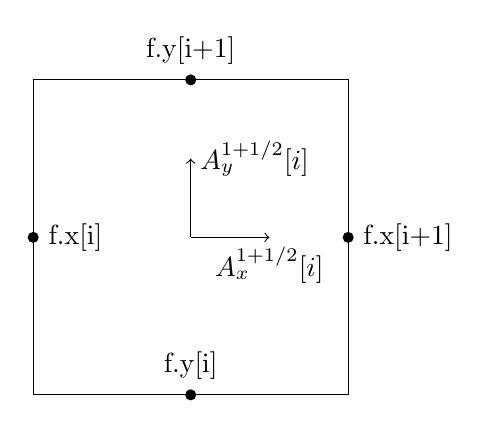
\begin{tikzpicture}[scale=1]
    \draw (-2,0)--(2,0)--(2,4)--(-2,4)--(-2,0);
    \fill (0,0) circle (2pt) node[above=2pt,fill=white]{f.y[i]};
    \fill (-2,2) circle (2pt) node[right=2pt,fill=white]{f.x[i]};
    \fill (0,4) circle (2pt) node[above=2pt,fill=white]{f.y[i+1]};
    \fill (2,2) circle (2pt) node[right=2pt,fill=white]{f.x[i+1]};
    \draw[->] (0,2)--(1,2) node[below]{$A^{1+1/2}_{x}[i]$};
    \draw[->] (0,2)--(0,3) node[anchor=west]{$A^{1+1/2}_{y}[i]$};
    \end{tikzpicture}
    \end{center}
    \caption{Basilisk存储示意}
\end{figure}
\mintinline[breaklines]{lexer.py:DiffLexer -x}{vector A[]}等命令可以在单元中心存储向量或标量值。由上文得$ \mathbf{U}^n, \nabla \Phi, \Phi^n$存储在网格中心,由他们计算得到的$\Phi^{n+1/2}_d$则储存在网格面上。相应的,Basilisk的交错网格直接存储的就是下一步计算所需的$u_d^{n+1/2}$。\par
回归算法本身,当我们求解一个标量的对流方程时,tracer flux会首先计算出位于每个单元面上的分量值即
\begin{equation}
    flux = u^{n+ \frac{1}{2}}_d \Phi^{n+ \frac{1}{2}}_d
\end{equation}
如下图:
\begin{figure}[H]
    \centering
    \begin{center}
    \begin{tikzpicture}[scale=1]
    \draw (-2,0)--(2,0)--(2,4)--(-2,4)--(-2,0);
    \draw[->] (0,-0.25)--(0,0.75) node[anchor=west]{$flux_y[0]$};
    \draw[->] (-2.25,2.0)--(-1.25,2.0) node[anchor=west]{$flux_x[0]$};
    \draw[->] (0,3.75)--(0,4.75) node[anchor=west]{$flux_y[1]$};
    \draw[->] (1.75,2)--(2.75,2) node[anchor=west]{$flux_x[1]$};
    \end{tikzpicture}
    \end{center}
    \caption{projection处理}
\end{figure}
而advection则会遍历每个方向求出相应的对流项值,同时求解对流方程直接返回$\Phi^{n+1}$\par
\textcolor{red}{出于工程及代码简洁性考虑,导致除物理量外,只能输如一个面上速度值作为参数,而根据前文的理论推导,我们需要位于$n,n+ \frac{1}{2}$时层的两个速度量,代码相应的做了简化,在advection函数中只能输入一个面单元速度,是故必须要在二者中选取一个时间层,例如在center.h中,选取的时间层就全部都位于$n+\frac{1}{2}$}
\subsection{tracer fluxes函数}\label{sec:tracer}
我们统一假设其输入的面上速度时层为第n时层则有
\begin{minted}[mathescape=true,breaklines]{lexer.py:DiffLexer -x}
/*本函数的目的在于采取上文中推导出的迎风格式计算$\mathbf{U}^{n+1/2}_i$,已知中心的速度场$f$保存在面中心的单元流量$uf$,源项$src$,计算时间步长$dt$,将最后的结果保存在每个单元表面中心上,指针为flux*/
void tracer_fluxes (
    scalar f,
    face vector uf,
    face vector flux,
    double dt,
    (const) scalar src)
{
 /*首先计算$\nabla f$,gradients()函数的目的是将第一个参数的梯度赋予第二个vector型函数中*/ 
  vector g[];
  gradients ({f}, {g});

/*接下来针对每一个面的中心计算$\Phi^{n+1/2}_d $,在这里我们将源项即压力项放置于src中并不进行单独计算*/
  foreach_face() {
/*首先是法相分量$ \Phi^n+\frac{\Delta}{2}min[1-\frac{\Delta t}{\Delta}u_i^{n},1]\frac{\partial \Phi^n}{\partial x_i}$*/

    double un = dt*uf.x[]/(fm.x[]*Delta + SEPS), s = sign(un);
    int i = -(s + 1.)/2.;
    double f2 = f[i] + (src[] + src[-1])*dt/4. + s*(1. - s*un)*g.x[i]*Delta/2.;

 /*其次计算$- \frac{\Delta t}{2}u_j^{n}\frac{\partial \Phi^n}{\partial x_j}$当为2维情况时该项只有一项,3维为两项,计算需要使用迎风格式*/

    #if dimension > 1
    if (fm.y[i] && fm.y[i,1]) {
      double vn = (uf.y[i] + uf.y[i,1])/(fm.y[i] + fm.y[i,1]);
      double fyy = vn < 0. ? f[i,1] - f[i] : f[i] - f[i,-1];
      f2 -= dt*vn*fyy/(2.*Delta);
    }
    #endif
    #if dimension > 2
    if (fm.z[i] && fm.z[i,0,1]) {
      double wn = (uf.z[i] + uf.z[i,0,1])/(fm.z[i] + fm.z[i,0,1]);
      double fzz = wn < 0. ? f[i,0,1] - f[i] : f[i] - f[i,0,-1];
      f2 -= dt*wn*fzz/(2.*Delta);
    }
    #endif

    flux.x[] = f2*uf.x[];
  }
  boundary_flux ({flux});
}
\end{minted}
将代码细节具体分析,在此以2D为例,暂不考虑网格自适应问题,假设研究网格与其邻近网格level值相等,得到:\par
\begin{center}
    \begin{tikzpicture}[scale=1]
    \draw[->] (-3,0) -- (3,0) node[anchor=north west] {x};%画出x轴并将最后的终结点其命名为x
    \draw[->] (0,-1) -- (0,3) node[anchor=south east] {y};%画出y轴并将最后的终结点其命名为y
    \draw[very thick,red]
        (0,0) -- (0,2.5);%在线段的中间添加标签,并使用fill = white使线条不透过标签
    \draw (-2.5,0) -- (-2.5,2.5)--(2.5,2.5)--(2.5,0);
    \fill [color = red] (0,1.25) circle (2pt) node[above=3pt,fill=white]{flux.x[i]};
    \fill (1.25,1.25) circle (2pt) node[right=2pt,fill=white]{f[i]};
    \fill (-1.25,1.25) circle (2pt) node[left=2pt,fill=white]{f[i-1]};
    \end{tikzpicture}
\end{center}
我们以x方向为例,上图中标红部分即为所求界面,中点为所求$\Phi^{n+1/2}_i$所在点\par
需要特别指出的是,在Basilisk中face vector型数据旨在每一个单元面中心定义数据,假设有face vector型数据$fv$,有单元中心点的坐标为$(i,j)$,那么$fv.x[]$所表示的面中心点的坐标为$(i-1/2,j)$,$fv.y[]$所表示的面中心点坐标为$(i,j-1/2)$。\par
以x方向为例,回顾源代码:\par
\mintinline{lexer.py:DiffLexer -x}{double un = dt*uf.x[]/(fm.x[]*Delta + SEPS), s = sign(un);} 其中un指代该方向上在单元中心的速度分量乘以时间步长除以网格长度,即$v_i^n\times \frac{\Delta t}{\Delta}$,SEPS是为了防止计算除零添加的备用项。\par
这里原本的算法应该是
\mintinline{lexer.py:DiffLexer -x}{dt*(uf.x[i] + uf.x[i+1])/((fm.x[] +fm.x[i+1])*Delta)},即使用位于该方向上的面元点进行平均计算单元中心位于时层$n$的速度分量,代码作者因为边界条件问题对其进行了简化。\par
此时会有三种情况,即$un>0,un<0,un=0$。\par
当$un>0$时,此时流动方向为:
\begin{center}
    \begin{tikzpicture}[scale=1]
    \draw[->] (-3,0) -- (3,0) node[anchor=north west] {x};%画出x轴并将最后的终结点其命名为x
    \draw[->] (0,-1) -- (0,3) node[anchor=south east] {y};%画出y轴并将最后的终结点其命名为y
    \draw[very thick,red]
        (0,0) -- (0,2.5);%在线段的中间添加标签,并使用fill = white使线条不透过标签
    \draw (-2.5,0) -- (-2.5,2.5)--(2.5,2.5)--(2.5,0);
    \fill [color = red] (0,1.25) circle (2pt) ;
    \fill (1.25,1.25) circle (2pt) node[above=2pt,fill=white]{f[i]};
    \fill (-1.25,1.25) circle (2pt) node[above=2pt,fill=white]{f[i-1]};
    \draw[->] (0.5,1.25) -- (2,1.25) node[below=2pt,fill=white]{un};
    \end{tikzpicture}
\end{center}
根据迎风格式,我们应该取中心点为$(i-1,j)$的单元对目标点进行拟合,根据代码\par
\mintinline[breaklines]{lexer.py:DiffLexer -x}{s = sign(un); int i = -(s + 1.)/2.;}
当$un>0$时$s = 1, i = -1$,将其带回最后$f2$表达式中:\par
\mintinline[breaklines]{lexer.py:DiffLexer -x}{double f2 = f[i] + (src[] + src[-1])*dt/4. + s*(1. - s*un)*g.x[i]*Delta/2.;}能满足针对单元$(i-1,j)$计算:
\begin{equation}
    f_2=f_{i-1}+\frac{\Delta}{2}[1-\frac{\Delta t}{\Delta}u_i^{n}]\frac{\partial f_{i-1}}{\partial x_i}
\end{equation}\par
而当$un<0$时,此时流动则变为:
\begin{center}
    \begin{tikzpicture}[scale=1]
    \draw[->] (-3,0) -- (3,0) node[anchor=north west] {x};%画出x轴并将最后的终结点其命名为x
    \draw[->] (0,-1) -- (0,3) node[anchor=south east] {y};%画出y轴并将最后的终结点其命名为y
    \draw[very thick,red]
        (0,0) -- (0,2.5);%在线段的中间添加标签,并使用fill = white使线条不透过标签
    \draw (-2.5,0) -- (-2.5,2.5)--(2.5,2.5)--(2.5,0);
    \fill [color = red] (0,1.25) circle (2pt) ;
    \fill (1.25,1.25) circle (2pt) node[above=2pt,fill=white]{f[i]};
    \fill (-1.25,1.25) circle (2pt) node[above=2pt,fill=white]{f[i-1]};
    \draw[->] (2,1.25) -- (0.5,1.25) node[below=2pt,fill=white]{un};
    \end{tikzpicture}
\end{center}
此时需要利用$(i,j)$迎风计算下风段的面中心点,需要注意的是,由于计算是由$(i,j)$反推
$(i-1/2,j)$,针对空间的差分应该取负号,代码满足关系式为:
\begin{equation}
    f_2=f_{i-1}+(-\frac{\Delta}{2})\frac{\partial f_{i-1}}{\partial x_i}-\frac{\Delta t}{\Delta}u_i^{n}\frac{\partial f_{i-1}}{\partial x_i}=f_{i-1}-\frac{\Delta}{2}[1+\frac{\Delta t}{\Delta}u_i^{n}]\frac{\partial f_{i-1}}{\partial x_i}
\end{equation}
以迎风格式处理完切向分量后,
最终我们得到$\Phi^{n+1/2}_i\times u^{n}_i$的近似式\mintinline[breaklines]{lexer.py:DiffLexer -x}{flux.x[] = f2*uf.x[];},近似式是因为:
\begin{enumerate}
    \item 该结果只保留了数值值,并没有考虑面的外法线方向正负
    \item $uf.x[]$并不是$u^{n+1/2}_i$的数值值,根据前文叙述其是位于第n时层的面上速度,且还需要除以网格单位长度
\end{enumerate}
\subsection{advection函数}\label{sec:advectionxijie}
首先值得注意的是本函数对tracer flux的应用,在tracer flux求出各个方向的$\Phi^{n+1/2}_d u^{n}_d$分量后,advection按照方向归类加和成$\mathbf{A^{n+\frac{1}{2}}}$的分量。\par
其次该函数目的是直接计算预测步的单元中心下一个时层的物理量$\Phi^{n+1}$
\begin{equation}
    \Phi^{n+1}=\Phi^n-\Delta t A^{n+1/2}
\end{equation}
其中$\Phi^n$已知,在代码中以$f[]$形式出现,而对于对流项,如下图
\begin{center}
    \begin{tikzpicture}[scale=1]
    \draw[->] (-3,0) -- (3,0) node[anchor=north west] {x};%画出x轴并将最后的终结点其命名为x
    \draw[->] (0,-1) -- (0,3) node[anchor=south east] {y};%画出y轴并将最后的终结点其命名为y
    \draw[very thick,red]
        (-1.25,0) -- (-1.25,2.5);%在线段的中间添加标签,并使用fill = white使线条不透过标签
    \draw (-1.25,2.5) -- (1.25,2.5)--(1.25,0);
    \fill [color = red] (-1.25,1.25) circle (2pt);
    \fill (1.25,1.25) circle (2pt);
    \draw[red][->] (-1.25,1.25) -- (-1.75,1.25);
    \draw[->] (1.25,1.25)--(1.75,1.25);
    \end{tikzpicture}
\end{center}
可以确定的是$flux.x[]$的数值因法相量与坐标轴方向相悖,在对流项中应取负值则有:
\begin{equation}
    \Phi^{n+1}(i)=f[i]-\frac{\Delta t}{\Delta}\sum_d (flux.x[i+1] - flux.x[i])
\end{equation}
表现为代码为:
\begin{minted}[mathescape=true,breaklines]{lexer.py:DiffLexer -x}
for (f,src in p.tracers,lsrc) {
    face vector flux[];
    tracer_fluxes (f, p.u, flux, p.dt, src);
    
foreach()
    foreach_dimension()
    f[] += p.dt*(flux.x[] - flux.x[1])/(Delta*cm[]);//注意f[]已经赋值了,$\Phi^{n+1}$被直接更新在$f[]$中了
\end{minted}

\section{附录:cneter.h中bcg格式的误差}
如前文所述,真正的代码构建的bcg.h方程为:
\begin{equation}
\mathbf{U}^{n+1/2}_d = \mathbf{U}^n+[\frac{\Delta}{2}-\frac{\Delta t}{2}u_i^{n+1/2}]\frac{\partial \mathbf{U}^n}{\partial x_d} - \frac{\Delta t}{2}u_j^{n+1/2}\frac{\partial \mathbf{U}^n}{\partial x_j}-\frac{\Delta t}{2}\nabla p^n
\end{equation}
其中$u_i^{n+1/2}$由式\ref{equ:euler}代表第一次标准计算得到,位于网格面中心,$n+1/2$时层上的速度。\par
根据测试及原文\cite{popinet2003gerris}可得,如果直接不对$ \mathbf{U}^{n+1/2}_d$进行迭代,而是直接使用计算而出的$u_i^{n+1/2}$,那么速度会在尖锐边界条件出产生强不稳定性。
\printbibliography[heading=bibintoc, title=\ebibname]
\end{document}
